\documentclass[12pt,a4paper]{report}

% --- Packages de base ---
\usepackage[utf8]{inputenc}
\usepackage[T1]{fontenc}
\usepackage[french]{babel}
\usepackage{graphicx}     % Pour les images
\usepackage{hyperref}     % Liens cliquables
\usepackage{geometry}     % Marges
\usepackage{amsmath,amssymb} % Maths si besoin
\usepackage{listings}     % Pour le code
\usepackage{color}
\usepackage{forest}
\usepackage{xcolor}
\usepackage{enumitem}
\usepackage{graphicx} % si pas déjà chargé
\usepackage{float}



% --- Marges ---
\geometry{
	a4paper,
	left=25mm,
	right=25mm,
	top=25mm,
	bottom=25mm
}

% --- Couleurs pour le code ---
\definecolor{codegray}{rgb}{0.5,0.5,0.5}
\definecolor{codepurple}{rgb}{0.58,0,0.82}
\definecolor{backcolour}{rgb}{0.95,0.95,0.95}

\lstdefinestyle{mystyle}{
	backgroundcolor=\color{backcolour},
	commentstyle=\color{codegray},
	keywordstyle=\color{blue},
	numberstyle=\tiny\color{codegray},
	stringstyle=\color{codepurple},
	basicstyle=\ttfamily\footnotesize,
	breaklines=true,
	frame=single,
	numbers=left,
	stepnumber=1,
	tabsize=2
}
\lstset{style=mystyle}

% --- Titre et auteur ---
\title{Documentation du projet OrganisX}
\author{Youssef Tghrayt}
\date{\today}

\begin{document}
	
	% --- Page de titre ---
	\maketitle
	
	% --- Préface ---
	\chapter*{Préface}

Ce document a pour objectif de présenter la conception et le développement de l'application \textbf{OrganisX}, une solution moderne de gestion de tâches basée sur \textbf{.NET 9} et \textbf{Angular}.

Il décrit l'architecture hexagonale choisie, l'organisation du backend et du frontend, ainsi que les communications entre microservices via RabbitMQ. 

Cette documentation est destinée à la fois aux développeurs qui souhaitent comprendre la structure du projet et aux parties prenantes qui souhaitent une vue globale de l'application.

\bigskip
\textit{Auteur : Youssef Tghrayt}

	
	% --- Table des matières ---
	\tableofcontents
	\newpage
	
	% --- Sections principales ---
	\chapter{Introduction}

Dans un contexte où la collaboration et la gestion efficace des tâches prennent une importance croissante, le projet \textbf{OrganisX} a pour objectif de fournir une solution moderne, modulaire et extensible permettant d’organiser le travail individuel et collectif. 

L’idée initiale est née du constat que les outils existants, bien que puissants, sont souvent soit trop complexes pour un usage personnel, soit trop limités pour un usage collaboratif en équipe. \textbf{OrganisX} se positionne comme un compromis entre simplicité et extensibilité, en mettant l’accent sur une architecture claire et évolutive.

\section{Objectifs du projet}
Les objectifs principaux du projet peuvent être résumés comme suit :
\begin{itemize}
	\item Proposer une application web simple et intuitive pour la gestion des tâches personnelles.
	\item Introduire progressivement des fonctionnalités collaboratives (partage, équipes, gestion de projets).
	\item Concevoir une architecture \textbf{hexagonale} afin de garantir une séparation claire entre le domaine métier, les services applicatifs et les couches d’infrastructure.
	\item Documenter systématiquement les choix techniques au travers des \textbf{ADR} (Architecture Decision Records).
	\item Mettre en place une feuille de route incrémentale basée sur des \textbf{MVP (Minimum Viable Products)} afin de livrer de la valeur rapidement et de manière continue.
\end{itemize}

\section{Approche et méthodologie}
La conception de \textbf{OrganisX} suit une approche incrémentale et agile :
\begin{itemize}
	\item Découpage du projet en trois MVP successifs : 
	\begin{enumerate}
		\item \textbf{MVP1} : gestion des tâches personnelles et authentification.
		\item \textbf{MVP2} : introduction de la collaboration (partage, équipes).
		\item \textbf{MVP3} : ajout de fonctionnalités avancées d’organisation (projets, notifications, reporting).
	\end{enumerate}
	\item Utilisation de \textbf{GitHub} pour le suivi des tâches (issues, milestones, projects).
	\item Documentation vivante et centralisée dans le projet \textbf{OrganisXDocs}, structurée en sections thématiques (architecture, backend, frontend, etc.).
\end{itemize}

\section{Vision à long terme}
Au-delà des trois premiers MVP, \textbf{OrganisX} vise à devenir une plateforme extensible qui pourra accueillir des modules additionnels tels que la gestion des ressources, l’intégration avec des outils tiers (calendriers, messageries), ou encore l’analyse de la productivité grâce à des métriques et des tableaux de bord.

Ainsi, ce projet se veut à la fois un terrain d’expérimentation technique (architecture hexagonale, documentation structurée, microservices) et une solution concrète pouvant évoluer en fonction des besoins utilisateurs.

	\chapter{Documentation Fonctionnelle}

\section{Roadmap fonctionnelle}

Le développement d’OrganisX est prévu en trois MVPs successifs, permettant de livrer rapidement de la valeur tout en élargissant progressivement le périmètre fonctionnel.

\subsection{MVP 1 : Gestion personnelle}
\begin{itemize}
	\item Authentification sécurisée (JWT / OAuth2).
	\item Création, modification et suppression de tâches personnelles.
	\item Organisation par catégories simples.
\end{itemize}

\subsection{MVP 2 : Collaboration}
\begin{itemize}
	\item Partage de tâches et projets entre utilisateurs.
	\item Gestion des équipes et attribution de rôles.
	\item Historique des modifications et activité en temps réel.
\end{itemize}

\subsection{MVP 3 : Organisation avancée}
\begin{itemize}
	\item Création et gestion de projets complexes.
	\item Système complet de notifications (RabbitMQ) et alertes personnalisées.
	\item Reporting et statistiques d’activité.
\end{itemize}










	\chapter{Cahier des charges - MVP 1}

\section{Introduction}
Le premier MVP (Minimum Viable Product) du projet \textbf{OrganisX} vise à développer une application web simple de gestion de tâches personnelles (type Todo list). 
Ce MVP permettra de valider les choix techniques, d’expérimenter l’architecture hexagonale mise en place et de tester l’expérience utilisateur de base avant d’ajouter des fonctionnalités avancées (notifications, paiements, gestion d’équipes, etc.).

\section{Objectifs du MVP 1}
\begin{itemize}
	\item Fournir un système d’authentification basique (inscription et connexion).
	\item Permettre à un utilisateur connecté de créer, consulter, modifier et supprimer ses propres tâches.
	\item Assurer une séparation claire entre le frontend (Angular) et le backend (ASP.NET Core en architecture hexagonale).
	\item Préparer le terrain pour l’évolutivité (microservices futurs, ajout d’équipes, etc.).
\end{itemize}

\section{Périmètre fonctionnel}
Le MVP 1 inclut uniquement les fonctionnalités essentielles listées ci-dessous.

\subsection{Périmètre, acteurs et scénarios}
\subsubsection{Acteurs principaux}
\begin{tabular}{|l|p{10cm}|}
	\hline
	\textbf{Acteur} & \textbf{Description} \\ \hline
	Utilisateur non authentifié & Peut s'inscrire ou se connecter \\ \hline
	Utilisateur authentifié & Gère ses tâches personnelles \\ \hline
	Système d'authentification & Émet et valide les jetons, applique les politiques de sécurité \\ \hline
\end{tabular}

\subsection{Cas d’utilisation principaux}
\begin{itemize}
	\item \textbf{UC1 - S’inscrire :} L’utilisateur crée un compte en fournissant un email et un mot de passe.
	\item \textbf{UC2 - Se connecter :} L’utilisateur accède à l’application via email et mot de passe. 
	\item \textbf{UC3 - Créer une tâche :} L’utilisateur ajoute une nouvelle tâche avec un titre, une description (optionnelle) et une date d’échéance.
	\item \textbf{UC4 - Lister mes tâches :} L’utilisateur visualise toutes ses tâches, triées par date de création ou échéance.
	\item \textbf{UC5 - Modifier une tâche :} L’utilisateur met à jour le titre, la description, l’échéance ou l’état d’une tâche (À faire, En cours, Terminé).
	\item \textbf{UC6 - Supprimer une tâche :} L’utilisateur supprime une tâche définitivement.
\end{itemize}

\subsection{Diagramme d’utilisation (optionnel)}
\begin{figure}[H]
	\centering
	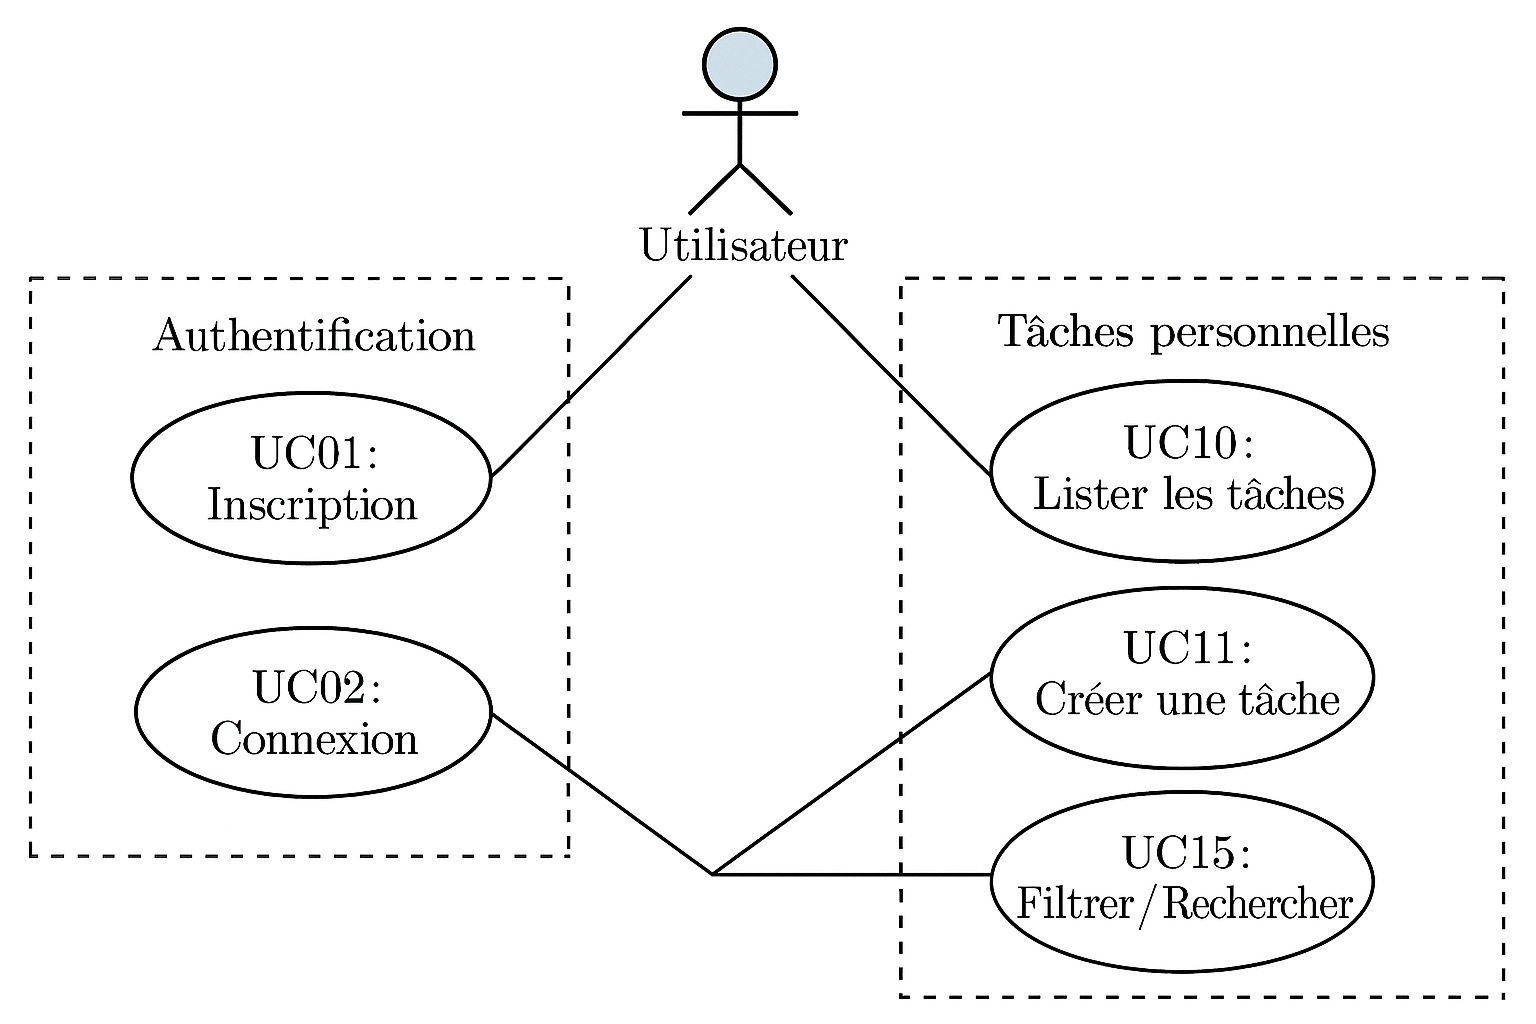
\includegraphics[width=0.8\textwidth]{images/diagram_use_cases.png}
	\caption{Diagramme des cas d’utilisation du MVP 1}
\end{figure}

\subsection{Paramètres et données}
\begin{itemize}
	\item \textbf{Personnalisation de l’affichage} : Choix du thème, langue et préférences d’interface.
	\item \textbf{Export des données} : Export des tâches au format CSV ou JSON.
\end{itemize}

\section{Exigences techniques}
\subsection{Backend}
\begin{itemize}
	\item Langage : C\# avec .NET 9.
	\item Architecture : Hexagonale (Domain, Application, Infrastructure, API).
	\item Base de données : PostgreSQL.
	\item Sécurité : Authentification JWT.
	\item Tests unitaires : xUnit.
\end{itemize}

\subsubsection{Modèle de données simplifié}
\begin{tabular}{|l|p{5cm}|p{6cm}|}
	\hline
	\textbf{Entité} & \textbf{Attributs} & \textbf{Contraintes} \\ \hline
	Utilisateur & id, email, passwordHash, displayName, locale, timeZone, createdAt & Email unique, mot de passe hashé \\ \hline
	Tâche & id, userId, title, description, status, priority, dueDate, tags[], createdAt, updatedAt & FK userId, taille max description 2000 caractères \\ \hline
\end{tabular}
\subsubsection{Diagramme de classes pour le microservice AuthService}
\begin{figure}[H]
	\centering
	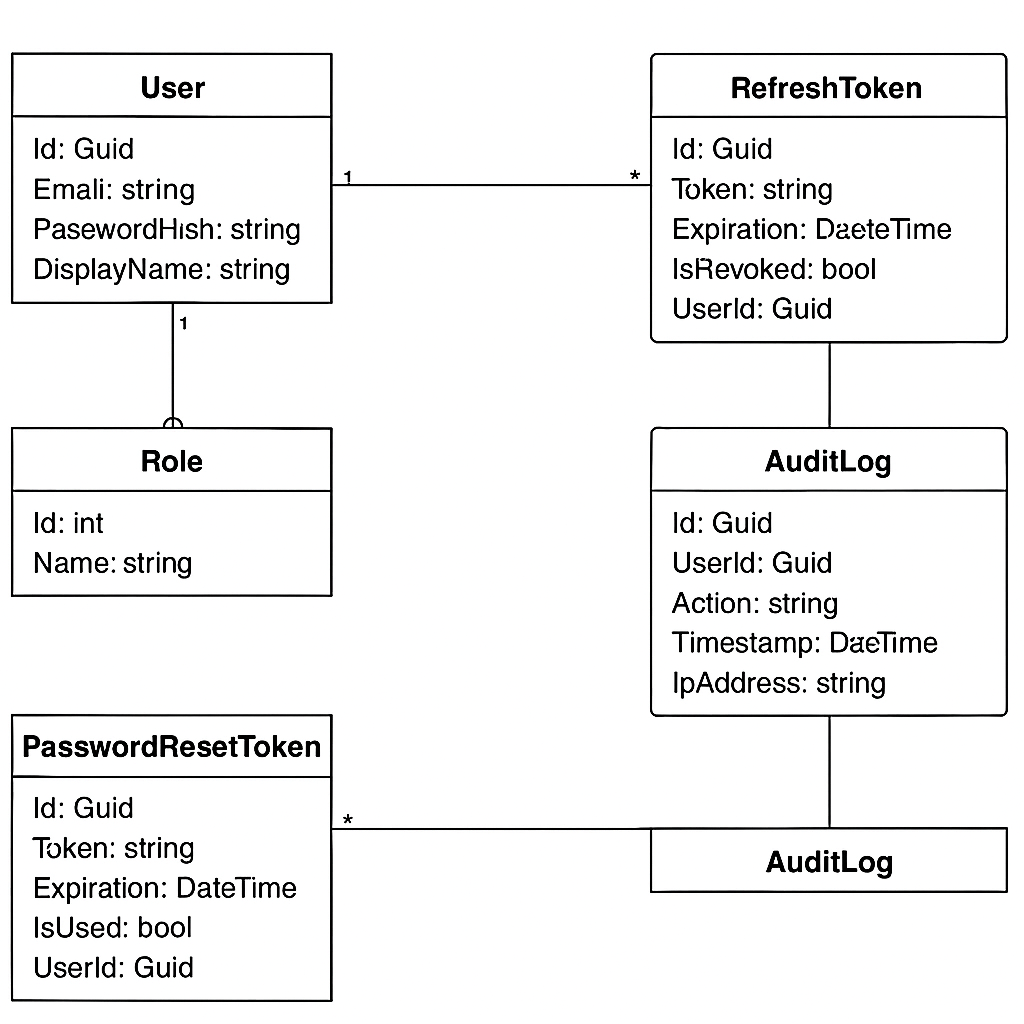
\includegraphics[width=0.5\textwidth]{images/MVP1_MCD.png}
	\caption{Diagramme de classes pour le microservice AuthService}
\end{figure}

\subsubsection{API principales}
\begin{description}
	\item[POST /api/v1/auth/register] Créer un compte.
	\item[POST /api/v1/auth/login] Obtenir tokens d'accès et de rafraîchissement.
	\item[GET /api/v1/tasks] Lister les tâches avec pagination et filtres.
	\item[POST /api/v1/tasks] Créer une tâche.
	\item[PUT /api/v1/tasks/\{id\}] Modifier une tâche.
	\item[DELETE /api/v1/tasks/\{id\}] Supprimer une tâche.
\end{description}

\subsection{Frontend}
\begin{itemize}
	\item Framework : Angular 20.
	\item Gestion d’état : services et RxJS.
	\item Communication : Appels HTTP vers l’API REST.
	\item UI : TailwindCSS ou Angular Material.
\end{itemize}

\section{Exigences non-fonctionnelles}
\begin{itemize}
	\item \textbf{Performance :} Les appels API doivent répondre en moins de 500ms en moyenne.
	\item \textbf{Sécurité :} Les mots de passe doivent être hashés (bcrypt).
	\item \textbf{Disponibilité :} 99\% pour MVP (mode développement).
	\item \textbf{Expérience utilisateur :} Interface simple et responsive.
	\item \textbf{Évolutivité :} Préparer la modularisation future (ajout de microservices).
\end{itemize}

\section{Architecture MVP 1}
\subsection{Backend}
\begin{itemize}
	\item \textbf{AuthService :} Gestion des comptes utilisateurs et authentification.
	\item \textbf{TodoService :} Gestion des tâches (CRUD).
\end{itemize}

\subsection{Frontend}
\begin{itemize}
	\item Module Auth (login, register).
	\item Module Todos (liste, création, édition, suppression).
	\item Shared components (header, forms, etc.).
\end{itemize}

\subsection{Schéma d’architecture}
\begin{figure}[H]
	\centering
	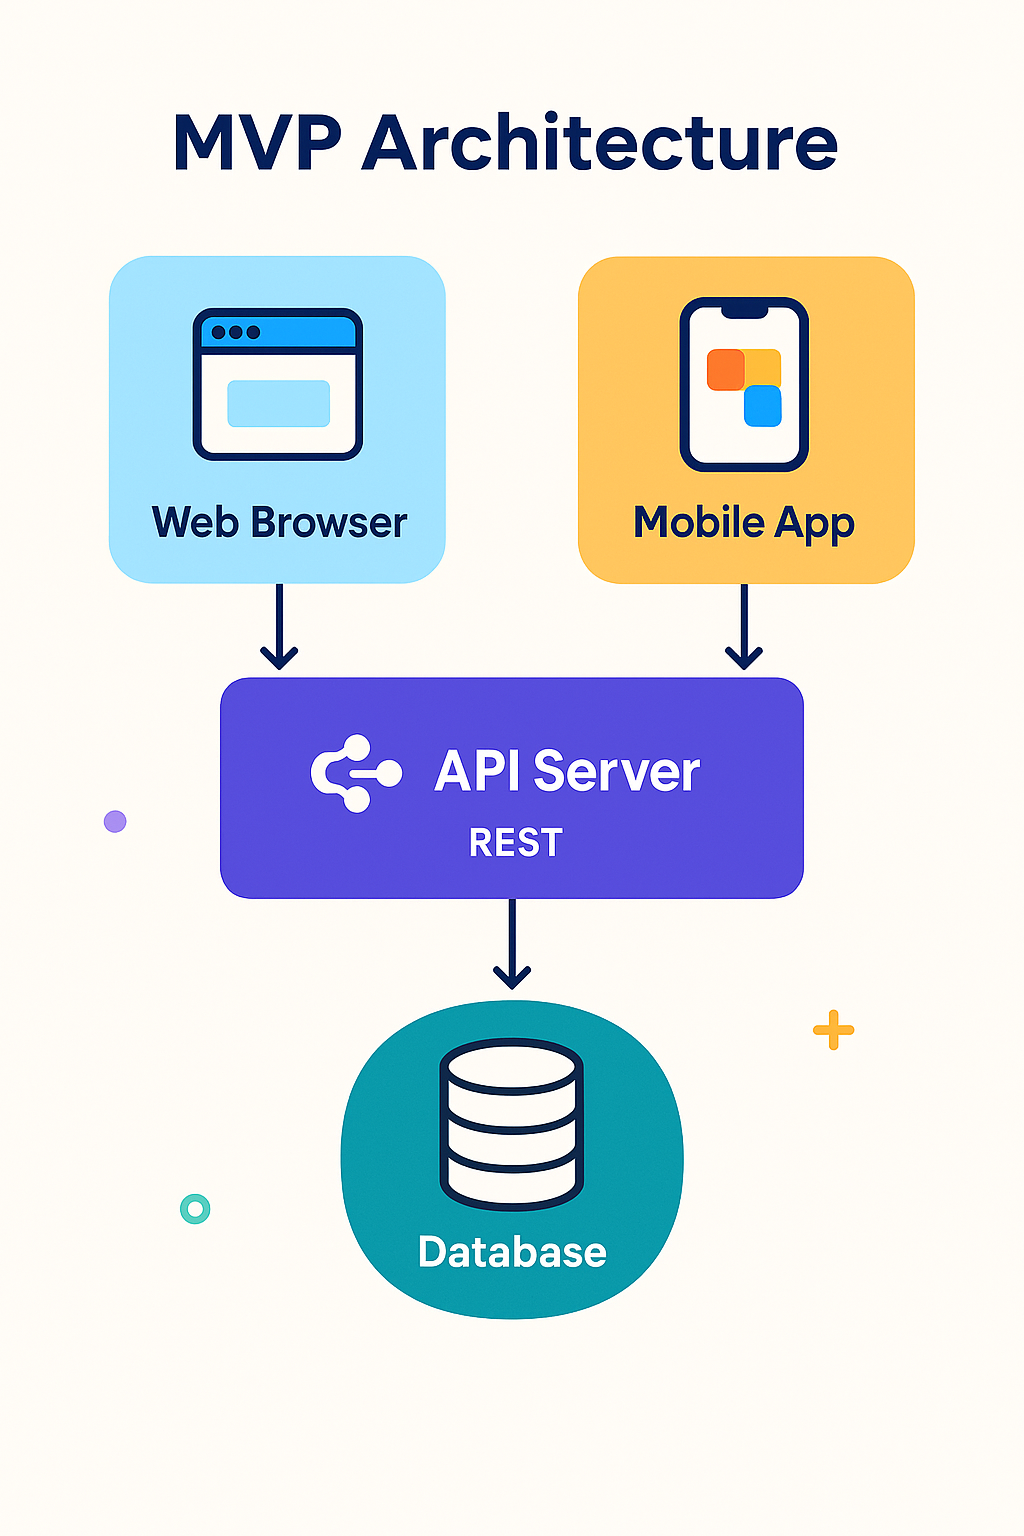
\includegraphics[width=0.5\textwidth]{images/Archi_mvp.png}
	\caption{Architecture technique du MVP 1}
\end{figure}

\section{Planification / Roadmap}
\begin{enumerate}
	\item \textbf{Semaine 1 :} Mise en place du projet backend (API .NET, PostgreSQL, AuthService). 
	\item \textbf{Semaine 2 :} Implémentation du TodoService (CRUD).
	\item \textbf{Semaine 3 :} Mise en place du frontend Angular (Auth, Todos).
	\item \textbf{Semaine 4 :} Intégration frontend-backend + tests utilisateurs.
\end{enumerate}
\subsection{Plan de tests}
\begin{itemize}
	\item Tests unitaires backend (Domain, Application).
	\item Tests intégration API Auth et Todo.
	\item E2E frontend : parcours inscription → création → complétion.
\end{itemize}

\subsection{Jalons MVP1}
\begin{enumerate}
	\item \textbf{Alpha} (S2-3) : Auth + création/liste tâches.
	\item \textbf{Beta} (S4-5) : Filtres/recherche, validations, tests intégration.
	\item \textbf{Release} (S6) : Durcissement sécurité, perfs, doc finalisée.
\end{enumerate}

\section{Conclusion}
Le MVP 1 permettra de valider la faisabilité technique du projet OrganisX et de fournir une base solide pour les fonctionnalités futures. L’approche incrémentale et modulaire garantit que chaque évolution du projet se construit sur des fondations fiables.

	\chapter{Architecture}

L’architecture du projet \textbf{OrganisX} constitue la fondation sur laquelle reposent toutes les fonctionnalités, la qualité et l’évolutivité du système. Elle a été conçue pour répondre aux besoins suivants :
\begin{itemize}
	\item Séparer clairement le \textbf{cœur métier} des préoccupations techniques.
	\item Assurer une \textbf{testabilité élevée} et faciliter la maintenance.
	\item Permettre une \textbf{évolution progressive} vers des solutions distribuées et scalables (microservices, cloud).
	\item Favoriser l’\textbf{adaptabilité technologique} (pouvoir remplacer une base de données, un framework, une librairie sans réécrire la logique métier).
\end{itemize}

\begin{figure}[h!]
	\centering
	\includegraphics[width=0.9\textwidth]{images/architecture.png}
	\caption{Architecture globale du projet OrganisX}
	\label{fig:architecture}
\end{figure}

\section{Philosophie générale}
Le projet adopte une approche \textbf{hexagonale} (également appelée \textit{Ports \& Adapters}).  
Cette architecture permet d’organiser le code autour de son \textbf{domaine métier}, tout en rendant les dépendances techniques secondaires et interchangeables.  
En pratique, cela signifie que le cœur applicatif (les règles métier et les cas d’utilisation) ne dépend d’aucune technologie particulière, mais uniquement d’interfaces (ports). Les implémentations concrètes (adapters) se trouvent en périphérie.

\newpage
\section{Structure Backend}
Le backend est développé en \textbf{.NET 9} et adopte une organisation orientée \textbf{microservices}, tout en respectant les principes de l’architecture hexagonale.  
Chaque service est indépendant, possède sa propre base de données et expose une API REST.  

Les microservices principaux sont :  
\begin{itemize}
	\item \texttt{OrganisX.AuthService} :
	\begin{itemize}
		\item Gestion de l’authentification et de l’autorisation via \textbf{JWT}.
		\item Contient les entités liées aux utilisateurs (User, Role).
		\item Peut être remplacé à terme par une solution externe (Azure AD, Keycloak).
	\end{itemize}
	
	\item \texttt{OrganisX.TaskService} :
	\begin{itemize}
		\item Gestion du cycle de vie des tâches (création, assignation, suivi).
		\item Implémente les règles métier associées (une tâche doit avoir un responsable, des deadlines, etc.).
	\end{itemize}
	
	\item \texttt{OrganisX.TeamService} :
	\begin{itemize}
		\item Gestion des équipes et des relations entre membres.
		\item Coordination avec \texttt{TaskService} pour affecter les tâches aux bons utilisateurs.
	\end{itemize}
	
	\item \texttt{OrganisX.ReportingService} (optionnel/futur) :
	\begin{itemize}
		\item Génération de rapports (productivité, suivi des tâches).
		\item Peut consommer des événements provenant des autres microservices.
	\end{itemize}
\end{itemize}

Chaque microservice respecte la structure interne suivante (dérivée de l’architecture hexagonale) :  
\begin{itemize}
	\item \textbf{Domain} : entités métier et invariants.
	\item \textbf{Application} : cas d’utilisation.
	\item \textbf{Infrastructure} : persistance, messaging (RabbitMQ/Azure Service Bus), accès API externes.
	\item \textbf{Api} : contrôleurs REST exposant les fonctionnalités.
\end{itemize}

La communication entre microservices peut se faire :  
\begin{itemize}
	\item en \textbf{synchrones} (API REST) pour les appels directs,
	\item en \textbf{asynchrones} (bus de messages) pour les événements métier (ex. création d’une tâche notifiant le service d’équipe).
\end{itemize}


\texttt{Domain}, \texttt{Application}, \texttt{Infrastructure} et \texttt{Api}.  

\begin{forest}
	for tree={
		font=\ttfamily,
		grow'=0,
		child anchor=west,
		parent anchor=south,
		anchor=west,
		calign=first,
		edge path={
			\noexpand\path [draw, \forestoption{edge}] (!u.south west) +(7.5pt,0) |- (.child anchor)\forestoption{edge label};
		},
		before typesetting nodes={
			if n=1
			{insert before={[,phantom]}}
			{}
		},
		fit=band,
		before computing xy={l=15pt},
	}
	[/backend
	[AuthService
	[AuthService.Domain]
	[AuthService.Application]
	[AuthService.Infrastructure]
	[AuthService.Api]
	]
	[TodoService
	[TodoService.Domain]
	[TodoService.Application]
	[TodoService.Infrastructure]
	[TodoService.Api]
	]
	[NotificationService
	[NotificationService.Domain]
	[NotificationService.Application]
	[NotificationService.Infrastructure]
	[NotificationService.Api]
	]
	[Shared
	[Shared]
	]
	]
\end{forest}

Cette organisation respecte le principe de \textbf{dépendances dirigées vers l’intérieur} : seul le domaine est indépendant, tandis que l’infrastructure dépend de l’application et du domaine.

\section{Structure Frontend}
Le frontend est conçu en \textbf{Angular 20}. Il constitue la porte d’entrée utilisateur vers les fonctionnalités d’OrganisX.  
Son organisation repose sur les principes suivants :
\begin{itemize}
	\item \textbf{Modules fonctionnels} : chaque domaine métier (authentification, gestion des tâches, gestion des équipes) est isolé dans un module Angular.
	\item \textbf{Services Angular} : centralisation de la logique de communication avec le backend via l’API REST.
	\item \textbf{Composants UI} : interfaces réactives permettant une bonne expérience utilisateur.
	\item \textbf{State management} (si besoin futur) : possibilité d’introduire NgRx pour gérer des flux complexes d’état.
\end{itemize}

\begin{forest}
	for tree={
		font=\ttfamily,
		grow'=0,
		child anchor=west,
		parent anchor=south,
		anchor=west,
		calign=first,
		edge path={
			\noexpand\path [draw, \forestoption{edge}] (!u.south west) +(7.5pt,0) |- (.child anchor)\forestoption{edge label};
		},
		before typesetting nodes={
			if n=1
			{insert before={[,phantom]}}
			{}
		},
		fit=band,
		before computing xy={l=15pt},
	}
	[/frontend
	[src/app
	[auth
	[login]
	[register]
	]
	[todos
	[task-list]
	[task-detail]
	[project-view]
	]
	[notifications
	[notification-list]
	]
	[shared
	[components]
	[services]
	]
	[core
	[interceptors]
	[guards]
	[api-clients]
	]
	]
	]
\end{forest}

\section{Communication Frontend/Backend}
L’interaction entre le frontend et le backend se fait via une \textbf{API RESTful}, en utilisant le format \textbf{JSON}.  
Quelques caractéristiques principales :
\begin{itemize}
	\item \textbf{Authentification} : sécurisée par \textbf{JWT}.
	\item \textbf{Endpoints REST} exposant les cas d’utilisation (ex. \texttt{POST /tasks}, \texttt{GET /teams}).
	\item \textbf{Validation et erreurs} : centralisées dans le backend et renvoyées au frontend pour affichage clair.
\end{itemize}

\section{Évolution future : vers les microservices}
Le projet démarre sous la forme d’un \textbf{monolithe modulaire}. Toutefois, grâce à l’architecture hexagonale, il est possible de faire évoluer certaines parties vers des \textbf{microservices indépendants} si la charge augmente.  
Par exemple :
\begin{itemize}
	\item Le module d’authentification peut être externalisé en un service dédié.
	\item La gestion des tâches peut être scalée indépendamment de la gestion des utilisateurs.
	\item La communication inter-services pourra s’appuyer sur des \textbf{messages asynchrones} (ex. RabbitMQ, Azure Service Bus).
\end{itemize}

Ainsi, l’architecture choisie garantit à la fois la \textbf{simplicité initiale} et la \textbf{scalabilité future}.

	\input{sections/backend.tex}
	\input{sections/frontend.tex}
	\input{sections/conclusion.tex}
	
\end{document}
